\chapter{SYSTEM DESIGN }

 \section{Use case model}
 \begin{figure}[H]
    \centering
    % Placeholder for a PDF/PNG exported use case diagram. 
    % Since we are using standard LaTeX, we describe the actor interactions.
    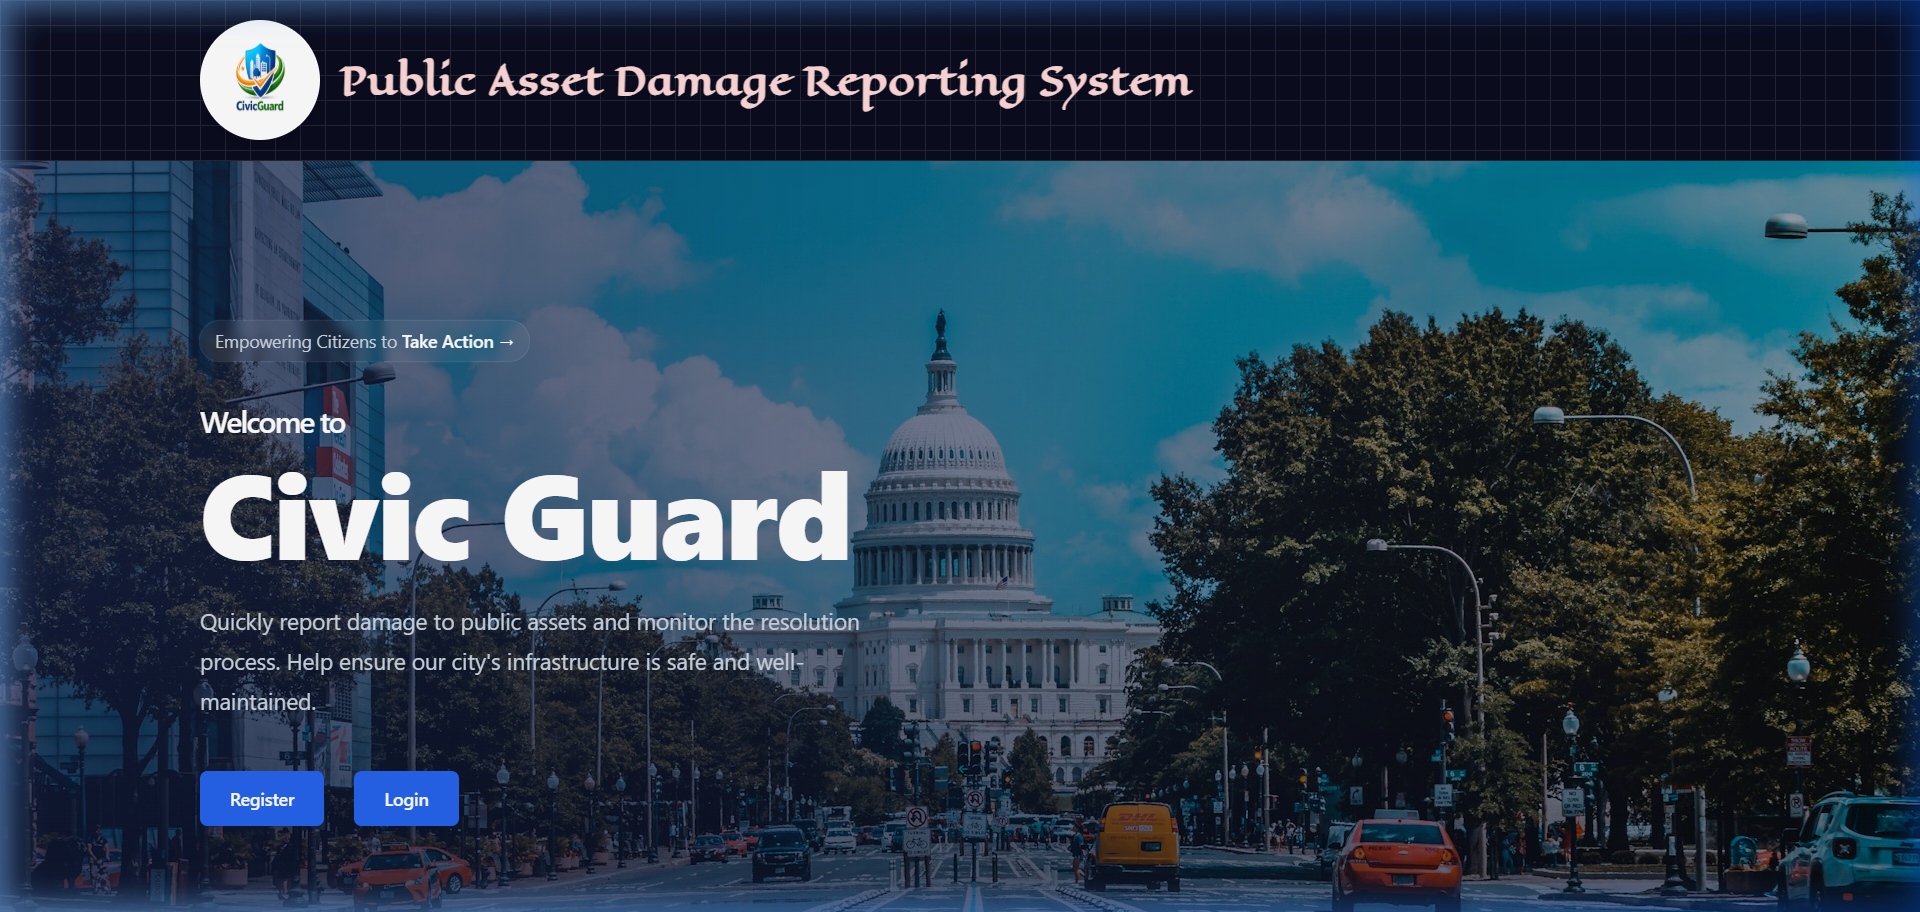
\includegraphics[width=1\textwidth,height=0.6\textwidth]{images/landing_page.png}
    \caption{System Interactions Overview}
\end{figure}
The Use Case model for CivicGuard captures the interactions between the three primary actors—Citizen, Department Officer, and Administrator—and the system's core functionalities. Citizens initiate the process by registering and submitting reports, while Officers and Admins facilitate the resolution and management of these reports.

 \section{Activity Diagram}
 \subsection{Report Lifecycle Flow}
 \begin{figure}[H]
    \centering
    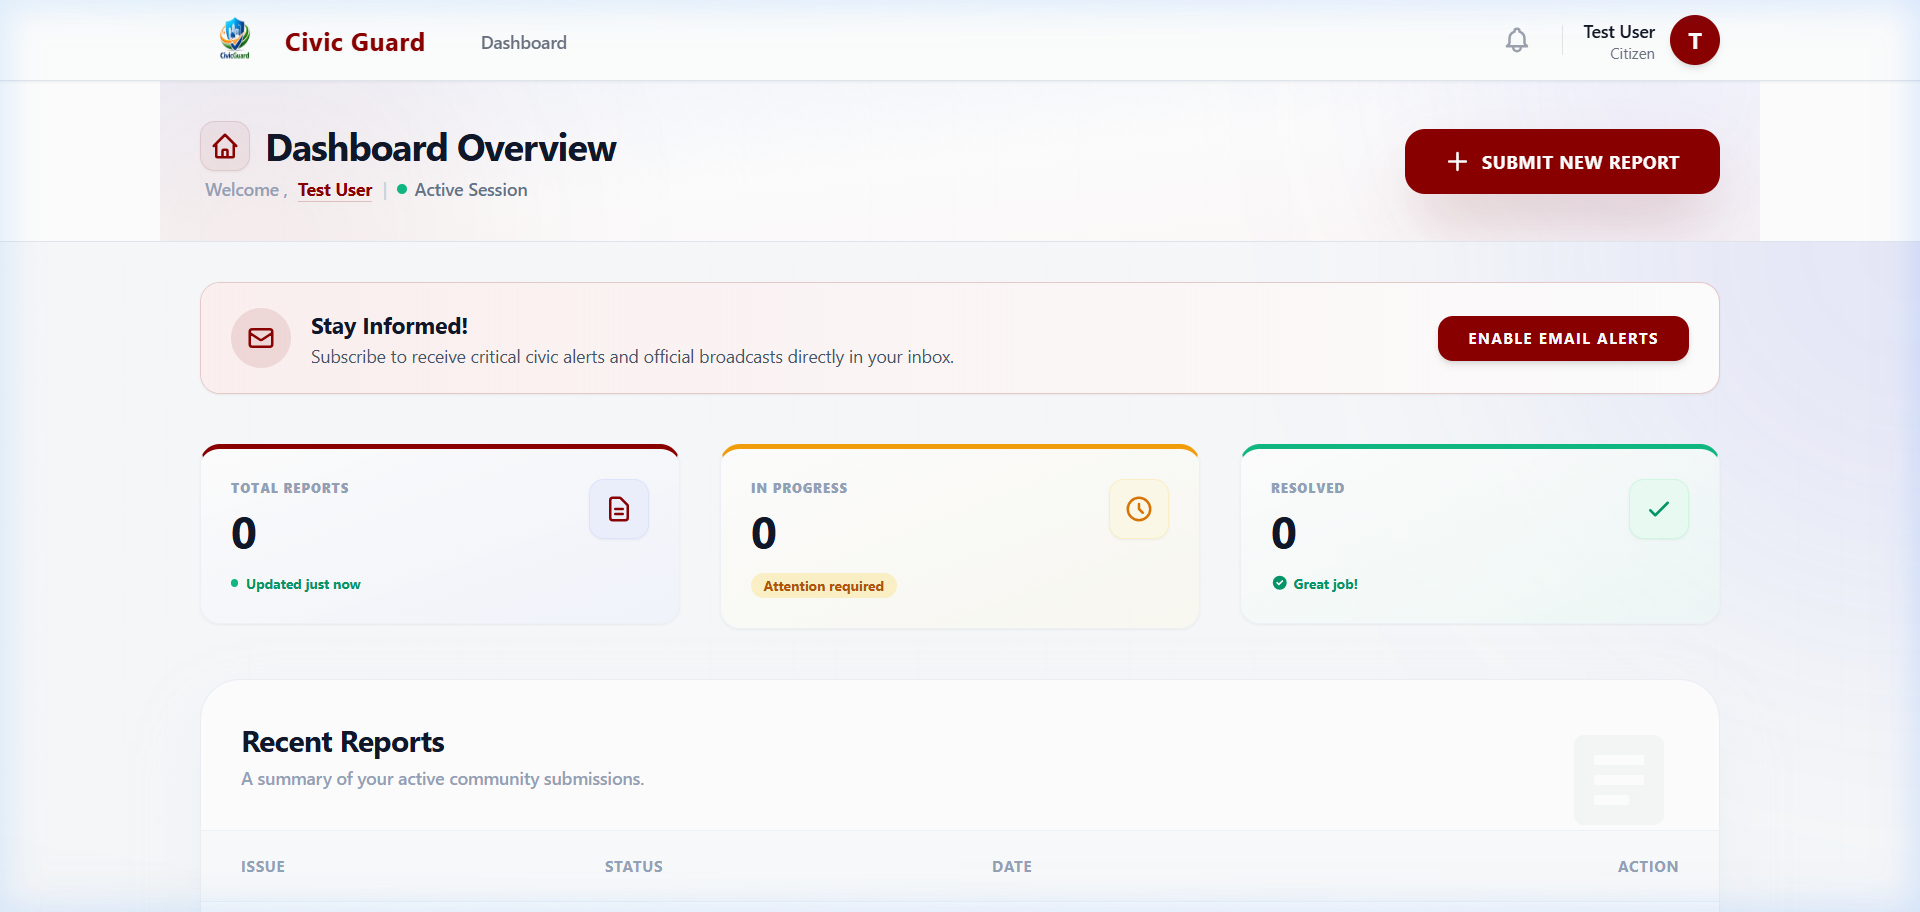
\includegraphics[width=0.8\textwidth]{images/dashboard.png}
    \caption{Activity Diagram - Report Progression}
\end{figure}
This diagram represents the flow of a report from submission to final resolution. It begins when a Citizen submits a report via the web interface. The system then enters a sorting state where it identifies the relevant department. Once assigned, the report enters a "Pending" state in the Officer's dashboard. The Officer then moves the report to "In Progress" when work begins. Finally, after uploading a resolution photo, the state changes to "Repaired", completing the cycle.

 \section{Project Design}
 CivicGuard's design focuses on transparency and ease of use. The UI is designed to be minimal yet informative, providing clear visual feedback through color-coded status badges and interactive dashboards. The backend design emphasizes scalability, using Laravel's robust routing and database patterns to handle thousands of reports and users concurrently.

 \subsection{UI Design}
 \begin{figure}[H]
    \centering
    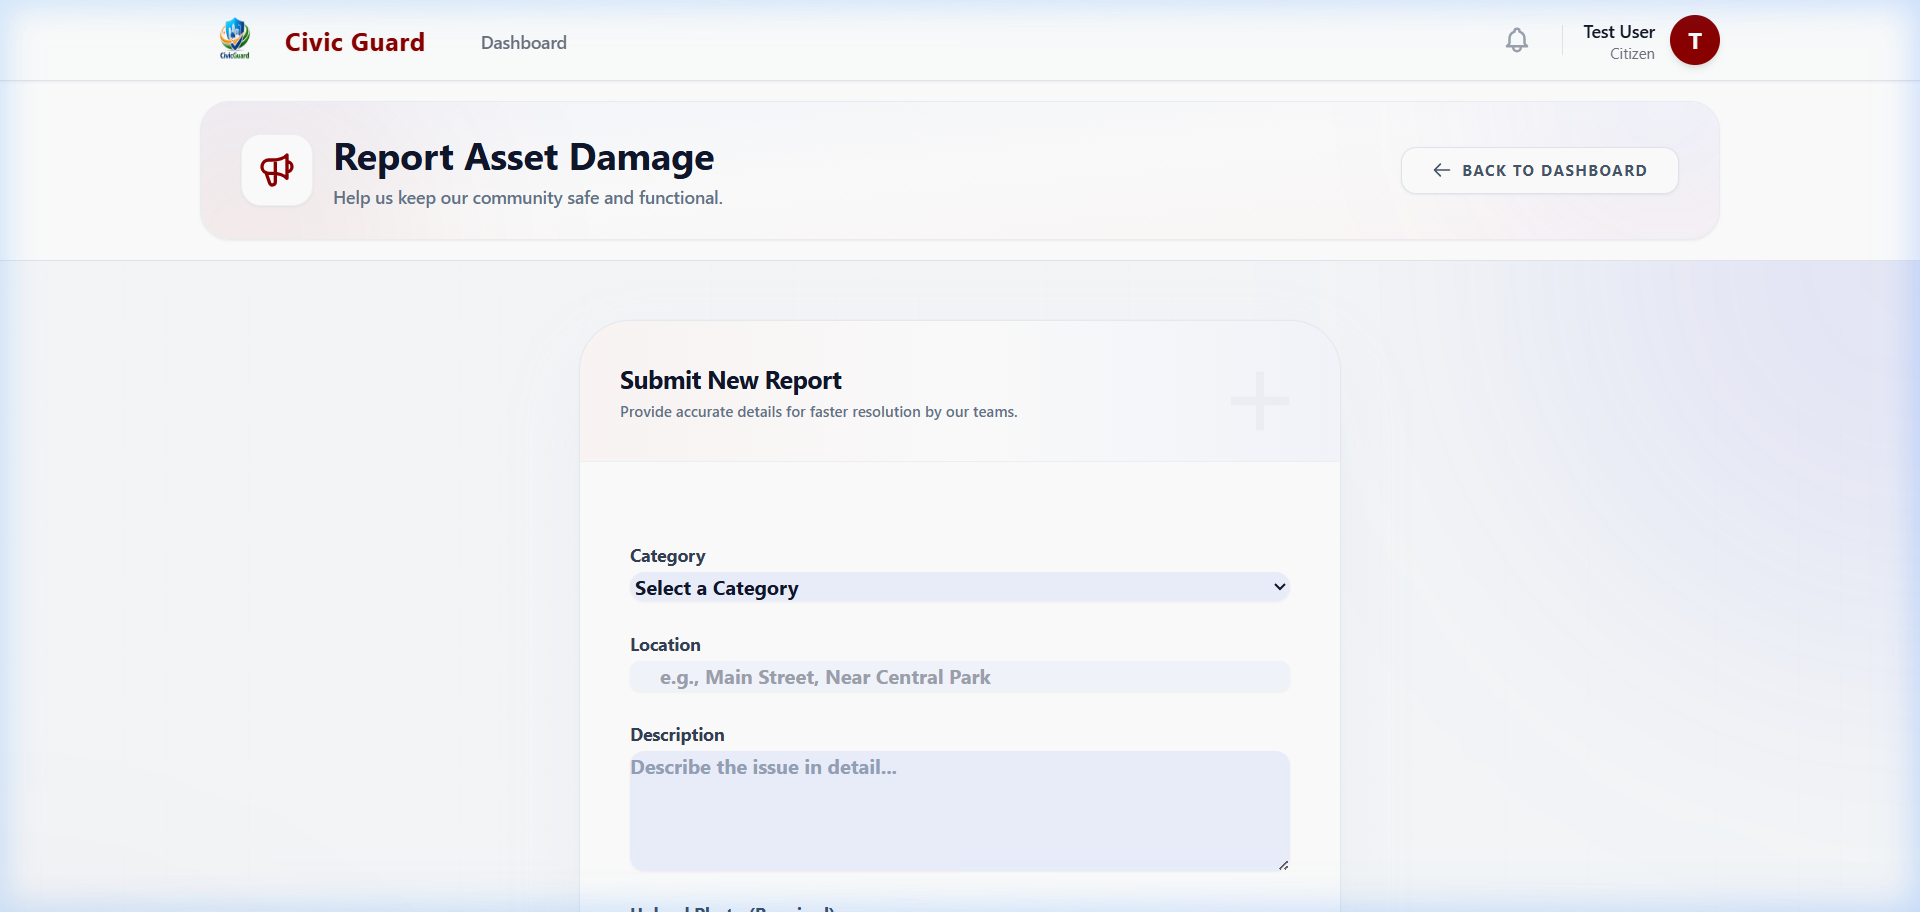
\includegraphics[width=0.8\textwidth]{images/report_creation.png}
    \caption{UI Design - Report Submission Form}
\end{figure}
The User Interface is built with a mobile-first approach using Tailwind CSS. The dashboard uses cards to represent different report states, providing a quick summary for users at a glance. Dark mode support and modern typography ensure a premium feel across all platforms.

 \subsection{Data Design}
 The database schema is designed for performance and data integrity. Key tables include:
 \begin{itemize}
    \item \texttt{users}: Stores account details, roles, and department tags.
    \item \texttt{reports}: Stores report content, category, location, and photo paths.
    \item \texttt{notifications}: Stores logs of all status updates and alerts.
 \end{itemize}

 \subsection{Question Design (Category Mapping)}
 Instead of simple questions, CivicGuard uses a Category Design to route complaints. These categories are mapped to specific departments within the application logic. 
\\\\
 \textbf{JSON Representation of Category Map}
 \begin{lstlisting}[style=phpstyle]
 [
    {
        "category": "Road Damage",
        "department": "Engineering & Public Works Department"
    },
    {
        "category": "Mosquito Issue",
        "department": "Health & Sanitation Department"
    },
    {
        "category": "Garbage Not Collected",
        "department": "Solid Waste Management Department"
    }
 ]
 \end{lstlisting}
This structure ensures that every complaint is handled by the correct authority without manual sorting.
